\subsection{Login}
The login sequence diagram presented in \ref{3img:[sequence]login} enable requesting user to access to the system checking the authenticity of the couple \textit{name} and \textit{password} stored in the Accounting Server. The user is logged and then he can normally works with the privilegies granted according to his position.

\begin{figure}[H]
\begin{centering}
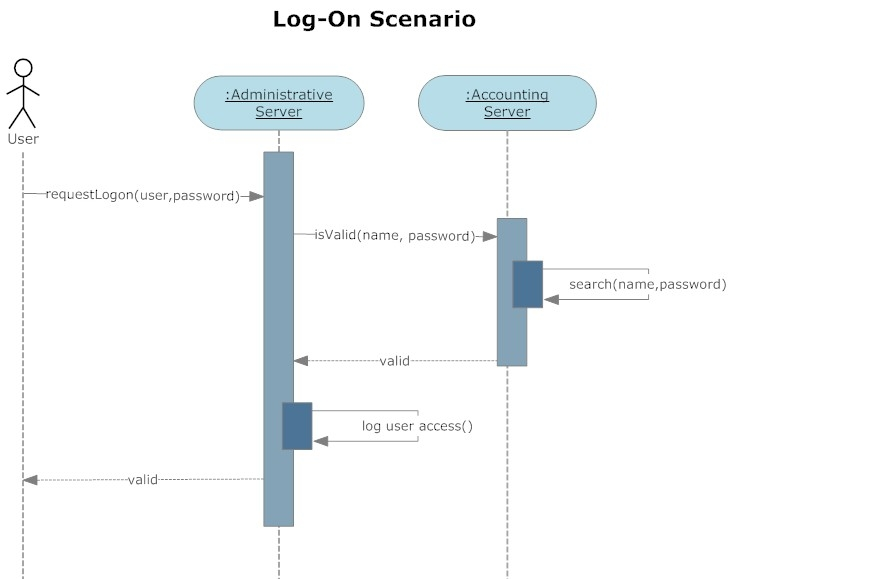
\includegraphics[scale=0.45]{assign3/sdraw/imgs/login.jpg}
\caption{Login sequence diagram.}
\label{3img:[sequence]login}
\end{centering}
\end{figure}


\subsection{Sending order}
The sending order sequence diagram locates the process aimed to complete the request, obtain the authorization to proceed and actually send it to the supplier chosen. In particular the Secretary is the main actor that perform the major part of the work and, once the order is completely filled with any kind of requested informations, the System provides to interrogate the CEO for sending definitively the order to the suppliers as showed in figure \ref{3img:[sequence]sending_order}.

\begin{figure}[H]
\begin{centering}
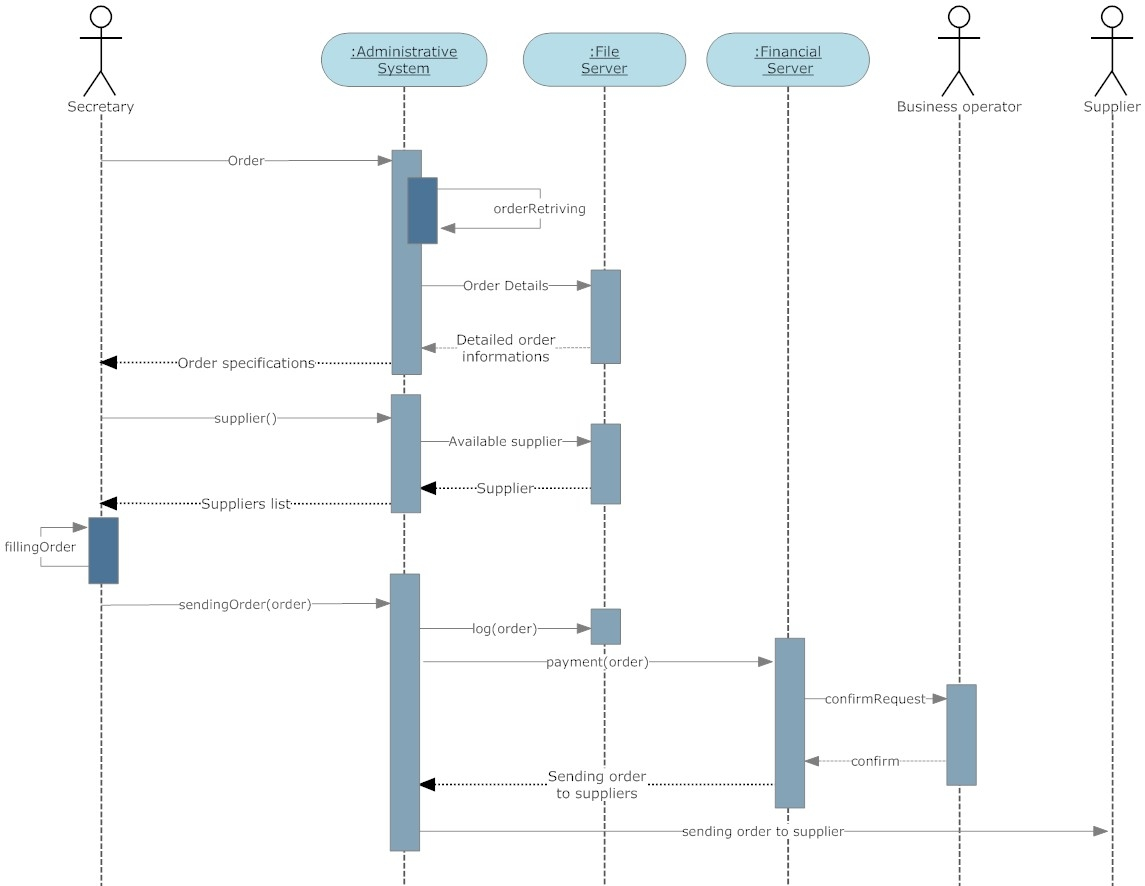
\includegraphics[scale=0.45,angle=90]{assign3/sdraw/imgs/sending_order.jpg}
\caption{Sending order sequence diagram.}
\label{3img:[sequence]sending_order}
\end{centering}
\end{figure}


\subsection{Maintenance schedule}
The maintenance schedule process can be divided in two distinct phases that are anyhow connected. Figure \ref{3img:[sequence]maintenance} illustrates ``Writing/Editing'' phase, that involves the System manager in the planning of the maintenance, and the second one, ``Expiration'' phase, reflects the ``presence'' of the System that contacts the System Manager at the moment the schedule time expires.

\begin{figure}[H]
\begin{centering}
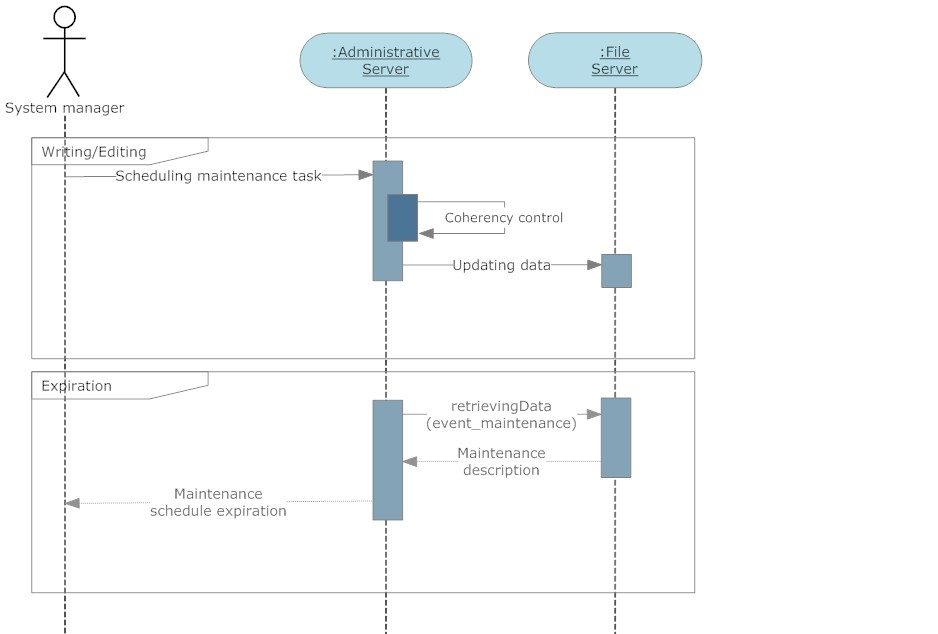
\includegraphics[scale=0.50]{assign3/sdraw/imgs/maintenance.jpg}
\caption{Maintenance schedule sequence diagram.}
\label{3img:[sequence]maintenance}
\end{centering}
\end{figure}


\subsection{Meeting management}
In order to schedule efficiently the working times, the time off, the marketing campaign and third meeting events, the Systems provide a function to manage the AllSpark meeting. In particular, coming from figure \ref{3img:[sequence]meeting}, the Secretary and the Representative are charged to involve the task and their exceptional counter-party is the Customer itself\footnote{For simplicity it is represented as customer, but as described in \ref{chap:Organization_focus} AllSpark has different kind of relations with several external entities.}.

Noteworthy is the bidirectional simplified ``Agreement with customer'' that may involve in different ways such as through mail, e-mail, telephone, chat and videoconference, depending on the previous ``Customer information'' gathered at the initial commercial relationships beginning.

\begin{figure}[H]
\begin{centering}
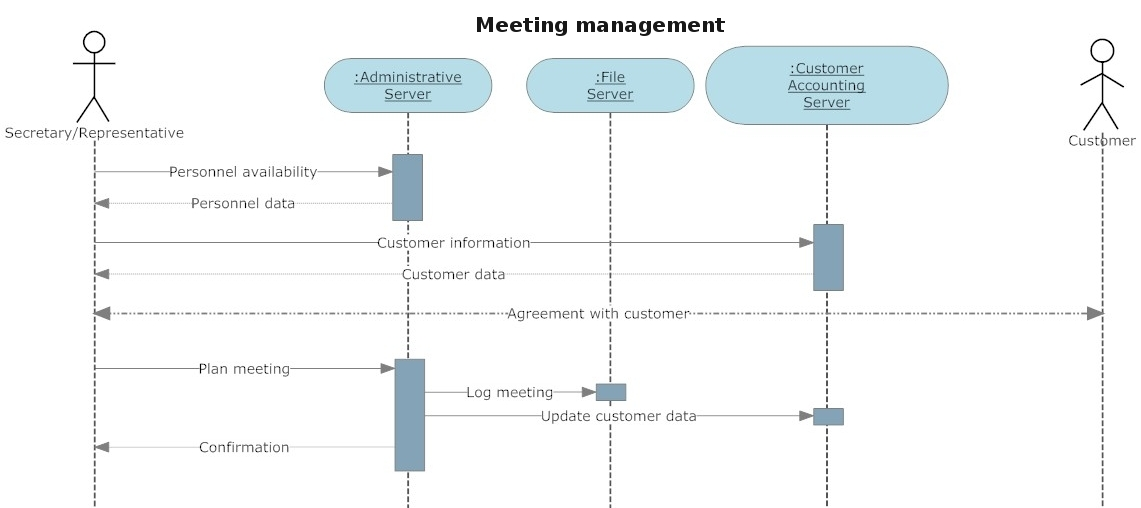
\includegraphics[scale=0.35]{assign3/sdraw/imgs/meeting.jpg}
\caption{Meeting management sequence diagram.}
\label{3img:[sequence]meeting}
\end{centering}
\end{figure}
